\documentclass[12pt,a4paper]{article}
\usepackage{geometry}
\geometry{a4paper,portrait,margin=1.4cm}
\usepackage[utf8]{inputenc}
\usepackage{amsmath}
\usepackage{amsfonts}
\usepackage{amssymb}
\usepackage{enumitem}
\usepackage{numprint}
\usepackage{graphicx}
\usepackage{caption}
\usepackage{gensymb}
\usepackage{fancyhdr}
\usepackage{csvsimple}
\usepackage{array}
\usepackage{wrapfig}
\usepackage{listings}
\usepackage{verbatim}
\usepackage{pdflscape}
\usepackage{siunitx}
\usepackage{listings}
\usepackage[svgnames]{xcolor}
\usepackage{xcolor}

\graphicspath{{./figures/}}
\pagestyle{fancy}
\fancyhf{}
\rhead{Candidate Number: 37443}
\lhead{2021/22 ST300 Project}
\cfoot{\thepage}
\setlength{\parindent}{0em}
\setlength{\parskip}{1em}
\lstset{language=R,
    breaklines=true,
    showstringspaces=false,
    basicstyle=\small\ttfamily,
    stringstyle=\color{DarkGreen},
    otherkeywords={0,1,2,3,4,5,6,7,8,9},
    morekeywords={TRUE,FALSE},
    deletekeywords={data,frame,length,as,character},
    keywordstyle=\color{blue},
    commentstyle=\color{DarkGreen},
    numbers=left,
    numberstyle=\ttfamily
}
\setlength\intextsep{0pt}


\definecolor{ttcolor}{RGB}{186,0,0}
\let\Oldtexttt\texttt
\renewcommand\texttt[1]{{\ttfamily\color{ttcolor}#1}}

\begin{document}
\begin{titlepage}
\vspace*{1cm}
\begin{center}
\Huge
\textbf{ST300}

\LARGE
Project

\vfill

\Large
Candidate Number: 37443

Session: 2021/22

\end{center}
\end{titlepage}
\section{Analysis}

\subsection{Data description}

The dataset analysed is the ''Countries of the World'' obtained on \textit{Kaggle}, containing 227 rows of data on economic and geographic variables of the countries and regions of the world, compiled between 2004 and 2010, as different countries perform census at different years, and certain types of data is only complied every 5 or 10 years.  The task is to propose model to explain the relationship between GDP per capita and the other variables in the dataset. We note that 48 rows contain missing values in one or more columns, which will be excluded in this analysis. This dataset contains the following variables:

Independent categorial variables: \texttt{Region}, which has 10 levels (originally 11, Baltic countries (of which there are 3) are recategorised as Eastern European countries) and \texttt{Climate} which has 6 levels. (Level 1 - Dry tropical or ice; 2 - Wet tropical; 3 - Temperate humid subtropical; 4 - Dry hot summers and wet winters. Levels in between (e.g. 1.5) also exist.)

Independent continuous variables: \texttt{Population}, \texttt{Area\_sqmi}, \texttt{Popdensity\_persqmi}, \texttt{Coastline},\\
 \texttt{Netmigration}, \texttt{Infantmorality\_per1k}, \texttt{Literacy}, \texttt{Phones\_per1k}, \texttt{Crops}, \texttt{Other}, \\
 \texttt{Birthrate}, \texttt{Deathrate}, \texttt{Agriculture}, \texttt{Industry}, \texttt{Service}. Note: \texttt{Crops} and \texttt{Other} sum to 1, where \texttt{Crops} represent the proportion of land cultivated for crops (including permenant crops);  similarly \texttt{Agriculture}, \texttt{Industry} and \texttt{Service} represent economic sector composition and sum to 1. 

Dependent (continuous) variable: \texttt{GDP\_pc}.

\subsection{Exploratory data analysis}

\begin{figure}[h]
\centering
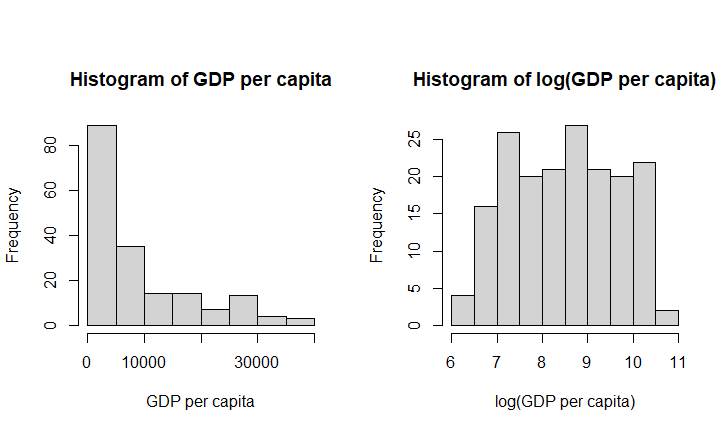
\includegraphics[width=0.8\linewidth]{histogram}
\caption{Histogram of GDP per capita}
\label{histogram}
\end{figure}

~\linebreak
Firstly, from the left-hand histogram in Figure \ref{histogram} we observe that the data is heavily right-skewed, which is to be expected in the context of GDP per capita of different countries. Hence, we perform a logarithmic transformation on the dependent variable to obtain a better spread of outcome data values. The results is shown in right-hand histogram in the same figure. 

\begin{figure}[h]
\centering
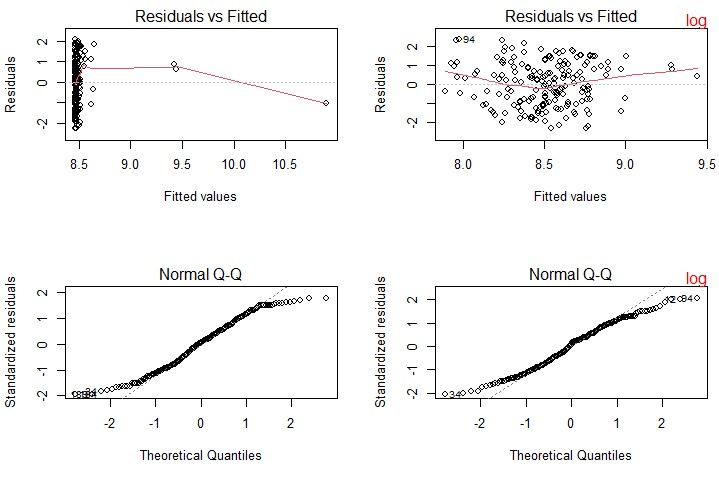
\includegraphics[width=1\linewidth]{log2}
\caption{Comparison of fit under logarithmic transformation}
\label{log}
\end{figure}

\pagebreak
We then identify the relationship between \texttt{log(GDP\_pc)} and each of the continuous variables separately. Table \ref{tablecor} in the appendix compares the correlation coefficient before and after a logarithmic transformation. In some cases, the correlation coefficient increases in magnitude significantly, for example for \texttt{population} it has increased in magnitude from -0.0141 to  -0.1651 under a logarithmic transformation; whereas in other cases it has led to a decrease in magnitude, for example \texttt{Literacy} decreased in magnitude from 0.6848 to 0.6499. 

Figure \ref{log} shows examples of improved fit after logarithmic transformations, indicating significantly better homoscedasticity as shown by the residuals-fitted plot, and normality deviation remains at an acceptable level as verified by the normal Q-Q plot. The two plots on the left refer to \texttt{Popdensity\_persqmi}, and the two plots on the right refer to \texttt{log(Popdensity\_persqmi)}. 

\subsection{Variable transformation}
Upon examining the relationship between \texttt{log(GDP\_pc)} and each of the continuous variables separately, subject to normality and homoscedasticity, as verified by the Residuals-Fitted and Normal Q-Q plots, \texttt{Population}, \texttt{Area\_sqmi}, \texttt{Popdensity\_persqmi}, \texttt{Infantmortality\_per1k}, \texttt{Phones\_per1k} will be transformed logarithmically.
 
As shown in Table 1, after the transformation, the correlation coefficient for these variables has increased in magnitude. Note that \texttt{Area\_sqmi} has a positive but near zero $r$-value before the transformation (0.0465), and larger but a negative $r$-value after the transformation (-0.2543). 

\subsection{Variable selection}
We initialy attempt to fit the model with all of independent variables. Perhaps surprisingly, this model has adjusted $R^2$ value 0.8786, and a near zero p-value for the F-statistic. However, examining each of the coefficients, most have an insignificant p-value for the t-statistic, as well as large standard errors for the estimate. 

To improve interpretability of this model, we attempt to improve the significance of these parameters, by only including a subset of the variables. We perform variable selection, using forward selection (FS) and backward elimination (BE) algorithms. The models produced by both algorithms are in agreement, with eight variables excluded: \texttt{Population}, \texttt{Area\_sqmi}, \texttt{Popdensity\_persqmi}, \texttt{Coastline}, \texttt{Climate}, \texttt{Literacy}, \texttt{Industry} and \texttt{Service}. 

We first compare the model with and without the seven continuous variables mentioned above (we will investigate the variable \texttt{Climate} seperately). The ANOVA test yields a p-value of 0.8867 for the F-statistic, along with a slight improvement to the adjusted $R^2$ value 0.8818. Therefore, we will drop these 7 variables. Next we investigate the categorical variable \texttt{Climate}. Again using an ANOVA test, the p-value is 0.7065 for the F-statistic, again with a slight improvement to the adjusted $R^2$ value 0.8833. Hence, we will also drop the variable \texttt{Climate}.

We note that many of the coefficients for the different levels of the categorical variable \texttt{Region} have relatively large standard errors and insignificant p-values for the t-statistic. An ANOVA test comparing models with and without the variable \texttt{Region} yields a p-value of 0.05037 for the F-statistic, which is weakly insignificant. However, we will retain this variable as otherwise we would have eliminated all categorial variables from our dataset. 

Finally, we investigate potentially multicolinear variables. First, we observe that the variables \texttt{Crops} and \texttt{Other}, representing land use decomposition of a country. By definition these two variables sum to 1, and observing the correlation matrix in Appendix \ref{cor}, these two variables are perfectly correlated (inversely), as expected. We compare the models with and without the variable \texttt{Other}. The ANOVA test yields a p-value of 0.01686 for the F-statistic. Hence we will drop the variable \texttt{Other}, as the value can be calculated from the other variable.

We also investigate possible multicollinearit between \texttt{Birthrate} and \texttt{Infantmortality\_per1k}. Again from the correlation matrix in Appendix \ref{cor}, the correlation coefficient between infant mortality rate and birthrate is 0.8389, suggesting strong relationship between these two variables. Intuitively, infant mortality rate relates to both deathrate and birthrate, as high infant morality may led to giving birth to more infants if fewer infants are except to survive to adulthood, and similar contribute to deathrate if the population is relatively young with infant morality contributing heavily to the population deathrate. This effect is expected to be more prominent in least-developed and developing countries, and less so in developed countries, where healthcare systems maybe better. Again, we perform an ANOVA test comparing the models with and without both \texttt{Birthrate} and \texttt{Deathrate}. We obtain a p-value 0.0032 for the F-test, so we retain ths variable.

We then also examine multicollinearity using variance inflation factor (VIF) calculated by the \texttt{cars} package in R. The full table is presented in Table \ref{vif} in the appendix. All GVIF values are below 10. Hence, there is no significant concern of multicollinearity in this model. 

\pagebreak
\subsection{Model diagnostics}
Finally, we check the model for potential outliers by calculating Cook's distance, as shown in Figure \ref{cooks}. The red line represents a threshold of $\frac{4}{n}\approx 0.02$. In this plot, there are 14 observations that exceed this threshold. However, re-fitting the model without these points does indeed increases the adjusted $R^2$ value. (0.9137 without vs 0.8798 including these observations).

\begin{wrapfigure}[15]{r}{0.5\textwidth}
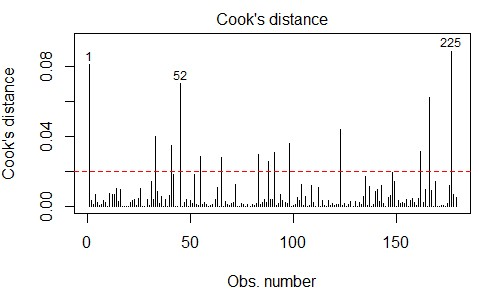
\includegraphics[width=1\linewidth]{cooks2}
\vspace{-10pt}
\caption{Cook's distance plot}
\label{cooks}
\end{wrapfigure}

Intuitively, outliers are to be expected due to the nature of the dataset, as the population size $n \approx 200$ is relative small. However, removing these observations may cause the model to be less representative since the dataset contained data of all countries. 

For example, the p-value for the t-statistic for the variable \texttt{Crops} has increased significantly from 0.0112 to 0.1154. Also if we removing these 14 observations, in addition to the 48 observations already removed due to incomplete date, we would have removed just under 30\% of the total number of observations, which is not ideal. Hence, we will retain all these observations to maintain the representativeness of the model.

\subsection{Checking model assumptions}
Finally, we verify the model assumptions are indeed not violated. From the left plot of Figure \ref{ass}, the standardised residuals appears to be scattered randomly above and below the zero line, and all lie within $\pm2$, suggesting constant variance of residuals. From the centre plot, all observations lie nowhere near the Cook's distance line, verifying that the outliers that we idenfitied in the previous section is not influential. From the right plot, although there is slightly bending tail on one end, it remains at an acceptable level so we confirm that normality is satisfied. Finally, we calculate the sum of residual errors to be $-3.3411 \times 10^{-15} \approx 0$, and mean of residual errors to be $-1.8677 \times 10^{-17} \approx 0$. Overall, we are convinced that the assumptions of a linear regression model are satisfied.

\begin{figure}[h]
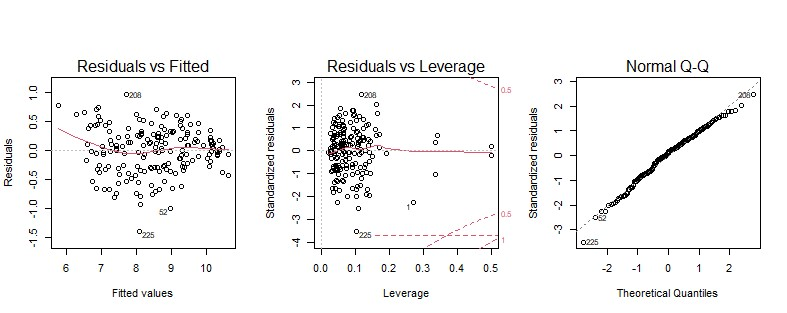
\includegraphics[width=1\linewidth]{final3}
\caption{Residuals-fitted, residuals-leverage and normal Q-Q plots}
\label{ass}
\end{figure}

\pagebreak
\subsection{Final model} \label{model}
The model proposed is as follows: 
\begin{multline*}
\log(\text{GDPpc}) =9.2763 +\alpha +0.0232 \times \text{Nmig} - 0.3591 \times \log(\text{Inmor}) +0.2004 \times \log(\text{Phone}) + \\ 
- 0.5441 \times \text{Crops} - 0.0223 \times \text{Birth} +0.0240 \times \text{Death} - 1.2582 \times \text{Agri}
\end{multline*}

where $\alpha$ is a sum of indicator functions for the categorical variable \texttt{Region}, given below. 

Note: most variable names abbreviated. Nmig - \texttt{Netmigration}, Inmor - \texttt{Infantmortalty\_per1k},  \\ Phone - \texttt{Phones\_per1k}, Birth - \texttt{Birthrate}, Death - \texttt{Deathrate}, Agri - \texttt{Agriculture}.
\begin{multline*}
\alpha = 0.0483 \times \mathbf{1}_\text{Asia} -0.2766 \times \mathbf{1}_\text{CIS} - 0.0477 \times \mathbf{1}_\text{E.Europe} + 0.0332  \times \mathbf{1}_\text{L.America} + 0.2685 \times  \mathbf{1}_\text{NearEast} +\\ 
+ 0.1397 \times  \mathbf{1}_\text{N.Africa} + 0.7462  \times \mathbf{1}_\text{N.America} +0.1661 \times  \mathbf{1}_\text{Oceania} + 0.3296 \times  \mathbf{1}_\text{W.Europe}
\end{multline*}

Note: reference category Sub-Saharan Africa; Asia - Asia (Ex. Near East); CIS - Commonwealth of Independence States (mainly former Soviet Union states); L.America - Latin American and the Caribbean; E.Europe - Eastern Europe; N.Africa - Northern Africa; N.America - Northern America; W.Europe = Western Europe. 

Observing the results shown in Appendix \ref{finalmodel}, we note that this model has an adjust $R^2$ value of 0.8798, a F-statistic value of 82.44 with the associated p-value of less than $2.2 \times 10^{-16} \approx 0$. We also note that most of the variables are (or nearly) statistically significant ($\leq 0.05$), although for some of the categorial variables, some of the levels have relatively high p-values for the t-statistic. Nonetheless, the magnitude of standard errors of many of the coefficients is also much smaller (by one or more orders of magnitude) relative to the estimated coefficient. A summary is presented in Appendix \ref{finalmodel}.

\subsection{Interpretation of model parameters}
 Regarding the continuous variable \texttt{Netmigration}, defined as $\frac{\text{Number of Immigrants}-\text{Emigrants}}{0.5 \times (\text{Pop. at start of year}+\text{at end of year})} \times 1000$: keeping all other variables fixed, an 1 unit increase  in the net migration rate, on average, leads to a change in GDP per capita by a factor of $e^{0.0232}=1.0235$, equivalent to 2.35\% increase. 

Regarding the log-transformed continuous variable \texttt{Infantmortality\_per1k}, defined as the deaths of children under one year of age per 1,000 live births: keeping all other variables fixed, a 1\% increase in the infant mortality rate, on average, leads to a change in GDP per capita by a factor of $1.01^{-0.3591}=0.9964$, equivalent to 0.36\% decrease.

Regarding the log-transformed continuous variable \texttt{Phones\_per1k}, defined as mobile phones per 1,000 people: keeping all other variables fixed, a 0.01 unit (or 1\%) increase in the rate, on average, leads to a change in GDP per capita by a factor of $1.01^{0.2004}=1.0020$, equivalent to 0.20\% increase. 

Regarding the continuous variable \texttt{Crops}, defined as the proportion of land cultivated for growing crops: keeping all other variables fixed, a 0.01 unit (or 1\%) increase in proportion of land for permenant crops, on average, leads to a change in GDP per capita by a factor of $e^{0.01 \times -0.5441}=0.9946$, equivalent to 0.54\% decrease. 

Regarding the continuous variable \texttt{Birthrate}, defined as total number of live births per 1,000 population: keeping all other variables fixed, a 0.01 unit (or 1\%) increase in the birthrate, on average, leads to a change in GDP per capita by a factor of $e^{0.01 \times -0.0223}=0.9998$, equivalent to 0.02\% decrease.

Regarding the continuous variable \texttt{Deathrate}, defined as the number of deaths per 1,000 population: keeping all other variables fixed, a 0.01 unit (or 1\%) increase in the deathrate, on average, leads to a change in GDP per capita by a factor of $e^{0.01 \times 0.0240}=1.0002$, equivalent to 0.02\% increase.

Regarding the continuous variable \texttt{Agriculture}, defined as the proportion of GDP per capita generated by the Agricultural (or primary) sector: keeping all other variables fixed, a 0.01 unit (or 1\%) increase in the proportion, on average, leads to a change in GDP per capita by a factor of $e^{0.01 \times -1.2582}=0.9875$, equivalent to 1.25\% decrease.

Regarding the categorial variable \texttt{Region}, compared to a country being in Sub-Saharan Africa, keeping all other variables fixed, a country in:
\begin{itemize}[noitemsep,topsep=0pt]
\item Asia, on average, has GDP per capita higher by 4.95\% ($e^{0.0483}=1.0495$);
\item the CIS, on average, has GDP per capita lower by 24.16\% ($e^{-0.2766}=0.7584$);
\item Eastern Europe, on average, has GDP per capita lower by 4.66\% ($e^{-0.0477}=0.9534$);
\item Latin America \& Caribbean, on average, has GDP per capita higher by 3.38\% ($e^{0.0332}=1.0338$);
\item Near East, on average, has GDP per capita higher by 30.80\% ($e^{0.2685}=1.3080$);
\item Northern Africa, on average, has GDP per capita higher by 14.99\% ($e^{0.1397}=1.1499$);
\item North America, on average, has GDP per capita higher by 110.90\% ($e^{0.7462}=2.1090$);
\item Oceania, on average, has GDP per capita higher by 18.07\% ($e^{0.1661}=1.1807$);
\item Western Europe, on average, has GDP per capita higher by 39.04\% ($e^{0.3296}=1.3904$).
\end{itemize}

Judging by the sign of the coefficients, most seem to be in agreement with economic theory. For example, a higher net migration rate, is indicative of a country being attractive to people from other countries, which suggests that the country is more economically developed. Another example is that a lower infant mortality rate is indicative of better healthcare system, a common feature in more economically developed countries.

Finally, we observe that the variable \texttt{Agriculture} to be the most important continuous variable in this model. Again, according to the three-sector model in economic theory, economies generally shift its main focus from primary (agriculture) to secondary (industry), and finally to the tertiary sector (service). Thus, an agricultural based economy is strongly indicative of lower GDP per capita, again supporting the fact that this variable has the largest coefficient in magnitude.

\subsection{Model limitations and conclusion}
The main limitation of this model is the size being relatively small $\approx 200$, meaning that each individual observations may have a high influence on the estimated coefficients. In section 1.5 where we evaluated the Cook's distance plot, we decided the keep all the observations despite high Cook's distance, since we prefer the model being more representative. However, since changes in the variables measured in this dataset may change significantly over the years, the model will very likely be significantly different when comparing economic data from different years. Furthermore, the assumption that observations being independent may not be entirely valid, since the economy of one country may be significantly dependent on other countries, for example oil-producing countries. 

However, many of the variables were excluded in the final model. Although a simpler model improves the explainability of the model, some of the variables which intuitively may have some relationship to GDP per capita according to economic theory is excluded, for example \texttt{Literacy}, where economic theory suggests that a higher literacy rate is indicative of higher productivity, hence higher GDP per capita. Nonetheless, the interpretation of the model given above also mostly agree with economic theory. Overall, we conclude that the model is of a good fit of the data, and also can be interpreted easily to draw relationships regarding GDP per capita and the other variables in the dataset.

\pagebreak
\appendix
\section{Appendix}

\subsection{Comparision of correlation coefficients under log-transformation}
This table shows the correlation coefficient between the dependent variables \texttt{log(GDP\_pc)} and each of the continuous independent variables. The correlation matrix between each of the continuous independent variables is given in Appendix \ref{cor}. 

Where the table cell is empty, this means the transformation is inappropriate for this variable, due to zero values being sent to $-\infty$. Note, we could have also used a shifted logarithmic transformation, e.g. $\log(x+\epsilon)$. However, this is undesirable as a number of these variables have values in $[0,1]$; and also that for very small $\epsilon$, the magnitude of $\log(\epsilon)$ becomes increasingly large and negative; and futher, makes the model more complex to interpret.

\hfill

\begin{table}[ht]
\centering
\begin{tabular}{>{\ttfamily}r r r r }
  \hline
 & Raw & Log-transform \\ 
  \hline
Population & -0.0141 & -0.1651 \\ 
  Area\_sqmi & 0.0465 & -0.2543 \\ 
  Popdensity\_persqmi & 0.1759 & 0.2165 \\ 
  Coastline & 0.0466 &  \\ 
  Netmigration & 0.2396 &  \\ 
  Infantmortality\_per1k & -0.8292 & -0.8838 \\ 
  Literacy & 0.6848 & 0.6499 \\ 
  Phones\_per1k & 0.8473 & 0.8682 \\ 
  Crops & -0.0317 &  \\ 
  Other & 0.0317 & 0.0522 \\ 
  Birthrate & -0.8341 & -0.8324 \\ 
  Deathrate & -0.3968 & -0.4006 \\ 
  Agriculture & -0.7852 &  \\ 
  Industry & 0.1477 & 0.1339 \\ 
  Service & 0.5913 & 0.5250 \\ 
   \hline
\end{tabular}
\caption{Comparision of correlation coefficients under log-transformation}
\label{tablecor}
\end{table}

\subsection{Table of generalised variance inflation factor (GVIF)}
Table only include variables used in the final model.

\hfill

\begin{table}[ht]
\centering
\begin{tabular}{>{\ttfamily}r r r r}
  \hline
 & GVIF & Df & GVIF\verb|^|(1/(2*Df)) \\ 
  \hline
Region & 11.262875 & 9 & 1.143997 \\ 
  Netmigration & 1.335901 & 1 & 1.155812 \\ 
  Infantmortality\_per1k & 7.100051 & 1 & 2.664592 \\ 
  Phones\_per1k & 8.133274 & 1 & 2.851890 \\ 
  Crops & 1.240374 & 1 & 1.113721 \\ 
  Birthrate & 7.544744 & 1 & 2.746770 \\ 
  Deathrate & 2.621064 & 1 & 1.618970 \\ 
  Agriculture & 3.009943 & 1 & 1.734919 \\
   \hline
\end{tabular}
\caption{Table of generalised variance inflation factor (GVIF)}
\label{vif}
\end{table}

\pagebreak
\begin{landscape}
\subsection{Correlation matrix of independent continuous variables}
Correlation calculated after applying log-transformation to \texttt{Population}, \texttt{Area\_sqmi}, \texttt{Popdensity\_persqmi}, \texttt{Infantmortality\_per1k} and \texttt{Phones\_per1k}.
\begin{table}[ht]
\small
\centering
\begin{tabular}{r|rrrrrrrrrrrrrrr}
  \hline
  & Pop & Area & Popdn & Coast & Nmig & Inmor & Lit & Phone & Crops & Other & Birth & Death & Agri & Ind & Ser \\
\hline
Pop & 1.0000 & 0.8359 & -0.0296 & -0.3416 & 0.0779 & 0.1666 & -0.1884 & -0.2569 & 0.0588 & -0.0588 & 0.1062 & 0.1520 & 0.1657 & 0.2066 & -0.3220 \\ 
  Area & 0.8359 & 1.0000 & -0.5734 & -0.3875 & 0.0358 & 0.3078 & -0.2340 & -0.3530 & -0.2104 & 0.2104 & 0.2429 & 0.2634 & 0.2532 & 0.2372 & -0.4304 \\ 
  Popdn & -0.0296 & -0.5734 & 1.0000 & 0.1957 & 0.0510 & -0.3117 & 0.1447 & 0.2593 & 0.4710 & -0.4710 & -0.2837 & -0.2529 & -0.2135 & -0.1236 & 0.3031 \\ 
  Coast & -0.3416 & -0.3875 & 0.1957 & 1.0000 & -0.2416 & -0.0711 & 0.0996 & 0.1248 & 0.1371 & -0.1371 & -0.0635 & -0.1486 & -0.0323 & -0.1890 & 0.1900 \\ 
  Nmig & 0.0779 & 0.0358 & 0.0510 & -0.2416 & 1.0000 & -0.1643 & -0.0538 & 0.0457 & -0.2574 & 0.2574 & -0.0351 & 0.0428 & -0.0966 & -0.0044 & 0.0915 \\ 
  Inmor & 0.1666 & 0.3078 & -0.3117 & -0.0711 & -0.1643 & 1.0000 & -0.7036 & -0.8492 & -0.0902 & 0.0902 & 0.8389 & 0.4991 & 0.7184 & -0.0151 & -0.6428 \\ 
  Lit & -0.1884 & -0.2340 & 0.1447 & 0.0996 & -0.0538 & -0.7036 & 1.0000 & 0.7538 & 0.1012 & -0.1012 & -0.7883 & -0.4017 & -0.6205 & 0.1057 & 0.4744 \\ 
  Phone & -0.2569 & -0.3530 & 0.2593 & 0.1248 & 0.0457 & -0.8492 & 0.7538 & 1.0000 & 0.0793 & -0.0793 & -0.8803 & -0.5356 & -0.7903 & 0.0937 & 0.6413 \\ 
  Crops & 0.0588 & -0.2104 & 0.4710 & 0.1371 & -0.2574 & -0.0902 & 0.1012 & 0.0793 & 1.0000 & -1.0000 & -0.1240 & -0.0660 & 0.0271 & -0.1223 & 0.0815 \\ 
  Other & -0.0588 & 0.2104 & -0.4710 & -0.1371 & 0.2574 & 0.0902 & -0.1012 & -0.0793 & -1.0000 & 1.0000 & 0.1239 & 0.0660 & -0.0271 & 0.1223 & -0.0815 \\ 
  Birth & 0.1062 & 0.2429 & -0.2837 & -0.0635 & -0.0351 & 0.8389 & -0.7883 & -0.8803 & -0.1240 & 0.1239 & 1.0000 & 0.4462 & 0.7040 & -0.1205 & -0.5417 \\ 
  Death & 0.1520 & 0.2634 & -0.2529 & -0.1486 & 0.0428 & 0.4991 & -0.4017 & -0.5356 & -0.0660 & 0.0660 & 0.4462 & 1.0000 & 0.4164 & -0.0126 & -0.3662 \\ 
  Agri & 0.1657 & 0.2532 & -0.2135 & -0.0323 & -0.0966 & 0.7184 & -0.6205 & -0.7903 & 0.0271 & -0.0271 & 0.7040 & 0.4164 & 1.0000 & -0.3528 & -0.6135 \\ 
  Ind & 0.2066 & 0.2372 & -0.1236 & -0.1890 & -0.0044 & -0.0151 & 0.1057 & 0.0937 & -0.1223 & 0.1223 & -0.1205 & -0.0126 & -0.3528 & 1.0000 & -0.5214 \\ 
  Ser & -0.3220 & -0.4304 & 0.3031 & 0.1900 & 0.0915 & -0.6428 & 0.4744 & 0.6413 & 0.0815 & -0.0815 & -0.5417 & -0.3662 & -0.6135 & -0.5214 & 1.0000 \\
   \hline

   \hline
\end{tabular}
\caption{Correlation matrix of independent continuous variables}
\label{cor}
\end{table}

Note: most variable names abbreviated. Pop - \texttt{Population}, Area - \texttt{Area\_sqmi}, Popdn - \texttt{Popdensity\_persqmi}, Coast - \texttt{Coastline}, Nmig - \texttt{Netmigration}, \\ Inmor - \texttt{Infantmortalty\_per1k},  Lit - \texttt{Literacy}, Phone - \texttt{Phones\_per1k}, Birth - \texttt{Birthrate}, Death - \texttt{Deathrate}, Agri - \texttt{Agriculture}, Ind - \texttt{Industry}, Ser - \texttt{Service}.
\end{landscape}



\subsection{Summary of final model} \label{finalmodel}
\verbatiminput{modelfinal.txt}

\pagebreak
\section{R code}
\lstinputlisting[breaklines]{finalcode.R}

\end{document}